\documentclass[12pt]{article}
%\documentclass[conference]{IEEEtran}
\usepackage[utf8]{inputenc}
\usepackage{amsmath, amssymb, graphicx} % Include any packages you need
\usepackage{geometry} % For setting margins, if needed
\usepackage{cite}
\usepackage{amsmath,amssymb,amsfonts}
\usepackage{algorithmic}
\usepackage{graphicx}
\usepackage[normalem]{ulem}
\usepackage{multirow}
\usepackage{longtable}
\usepackage{hyperref}
\usepackage{xltabular}
\usepackage{textcomp}
\usepackage{xcolor}
\def\BibTeX{{\rm B\kern-.05em{\sc i\kern-.025em b}\kern-.08em
		T\kern-.1667em\lower.7ex\hbox{E}\kern-.125emX}}
\geometry{margin=1in} % Adjust as necessary

\title{Appendices}
\date{}
\begin{document}
	
	\maketitle
	\tableofcontents

	\appendix
%	\section {Appendices}
%	\newline
	\section{System Data}
	This section details the bus and line data used in the study.
	
	\subsection{5-Bus Test System}
	The total active power demand of this distribution system in Table \ref{tab:buslinedata5bus} is 400 kW. Table~\ref{tab:loadflowresult} compares the load flow results of the implemented BFS with published results. Running BFS on the 33-Bus yields solutions consistent with the published results in Bouchekara et al., 2020.
	
	\begin{table}[h!]
		\centering
		\caption{Bus and Line Data of a 5-Bus RDS}
		\vspace{10pt}
		\resizebox{\columnwidth}{!}{%
			\begin{tabular}{|cccccccc|}
				\hline
				\multicolumn{1}{|c|}{\multirow{2}*{\centering \begin{tabular}[c]{@{}c@{}}Line\\ No.\end{tabular}}} & 
				\multicolumn{1}{c|}{\multirow{2}{*}{\begin{tabular}[c]{@{}c@{}}Snd.\\ Bus\end{tabular}}} & 
				\multicolumn{1}{c|}{\multirow{2}{*}{\begin{tabular}[c]{@{}c@{}}Rcv. Bus\\ (Bus No.)\end{tabular}}} & \multicolumn{2}{c|}{Load at Rcv. Bus} & \multicolumn{2}{c|}{Line Impedance} & \multirow{2}*{\centering \begin{tabular}[c]{@{}c@{}}Imax\\ (Amps)\end{tabular}} \\ \cline{4-7}
				
				\multicolumn{1}{|c|}{} & \multicolumn{1}{c|}{} & \multicolumn{1}{c|}{} & \multicolumn{1}{c|}{P (kW)} & \multicolumn{1}{c|}{Q (kVAr)} & \multicolumn{1}{c|}{R (ohms)} & \multicolumn{1}{c|}{X (ohms)} &  \\ \hline
				\multicolumn{1}{|c|}{} & \multicolumn{1}{c|}{S/S} & \multicolumn{1}{c|}{1} & \multicolumn{1}{c|}{0} & \multicolumn{1}{c|}{0} & \multicolumn{1}{c|}{0} & \multicolumn{1}{c|}{0} & N/A \\ \hline
				\multicolumn{1}{|c|}{1} & \multicolumn{1}{c|}{1} & \multicolumn{1}{c|}{2} & \multicolumn{1}{c|}{100} & \multicolumn{1}{c|}{60} & \multicolumn{1}{c|}{0.0922} & \multicolumn{1}{c|}{0.0470} & 400 \\ \hline
				\multicolumn{1}{|c|}{2} & \multicolumn{1}{c|}{2} & \multicolumn{1}{c|}{3} & \multicolumn{1}{c|}{90} & \multicolumn{1}{c|}{40} & \multicolumn{1}{c|}{0.4930} & \multicolumn{1}{c|}{0.2510} & 400 \\ \hline
				\multicolumn{1}{|c|}{3} & \multicolumn{1}{c|}{3} & \multicolumn{1}{c|}{4} & \multicolumn{1}{c|}{120} & \multicolumn{1}{c|}{80} & \multicolumn{1}{c|}{0.3661} & \multicolumn{1}{c|}{0.1864} & 400 \\ \hline
				\multicolumn{1}{|c|}{4} & \multicolumn{1}{c|}{2} & \multicolumn{1}{c|}{5} & \multicolumn{1}{c|}{90} & \multicolumn{1}{c|}{40} & \multicolumn{1}{c|}{0.1640} & \multicolumn{1}{c|}{0.1564} & 400 \\ \hline
				\multicolumn{4}{|c|}{Base MVA: 100 MVA} & \multicolumn{4}{c|}{Base Voltage: 12.66 kV} \\ \hline
			\end{tabular}%
		}
		\label{tab:buslinedata5bus}
	\end{table}
	
	
	
	
	\begin{table}[htbp]
		\caption{Summary of IEEE 33-Bus Load Flow Analysis Results}
		\begin{center}
			\begin{tabular}{ccc}
				\hline
				\textbf{IEEE 33-Bus Test System} & \textbf{BFS} & \textbf{Bouchekara et al., 2020} \\ \hline
				Tot. Active Power Loss (kW)      & 202.6771     & 202.6771                   \\
				Tot. Reactive Power Loss (kVAr)  & 135.1410     & 135.1410                   \\
				Minimum Voltage (pu)             & 0.913        & 0.913                      \\
				Min. Voltage Bus Location        & Bus 18       & Bus 18                     \\	\hline
			\end{tabular}
			\label{tab:loadflowresult}
		\end{center}
	\end{table}
	
	\subsection{IEEE 33-Bus System}
	The total demand is 3.715 MW active and 2.3 MVAr reactive power. Table \ref{tab:33busdata} summarizes the bus and line data.
	
	\begin{table}[htbp]
		\centering
		\caption{Bus and Line Data of the IEEE33-Bus RDS}
		\vspace{5pt}
		\label{tab:33busdata}
		\tiny % Reduce font size
		\setlength{\tabcolsep}{5pt}
		\resizebox{\columnwidth}{!}{%
			\begin{tabular}{|ccccccccc|}
				\hline
				\multicolumn{1}{|c|}{\multirow{2}{*}{\textbf{\begin{tabular}[c]{@{}c@{}}Line \\ No.\end{tabular}}}} &
				\multicolumn{1}{c|}{\multirow{2}{*}{\textbf{\begin{tabular}[c]{@{}c@{}}Snd.\\ Bus\end{tabular}}}} &
				\multicolumn{1}{c|}{\multirow{2}{*}{\textbf{\begin{tabular}[c]{@{}c@{}}Rcv.\\ Bus\\ (Bus \\ no.)\end{tabular}}}} &
				\multicolumn{3}{c|}{\textbf{Load at Rcv. Bus}} &
				\multicolumn{2}{c|}{\textbf{\begin{tabular}[c]{@{}c@{}}Line \\ Impedance\end{tabular}}} &
				\multirow{2}{*}{\textbf{Imax}} \\ \cline{4-8}
				\multicolumn{1}{|c|}{} &
				\multicolumn{1}{c|}{} &
				\multicolumn{1}{c|}{} &
				\multicolumn{1}{c|}{\textbf{\begin{tabular}[c]{@{}c@{}}P\\ (kW)\end{tabular}}} &
				\multicolumn{1}{c|}{\textbf{\begin{tabular}[c]{@{}c@{}}Q\\ (kVAr)\end{tabular}}} &
				\multicolumn{1}{c|}{\textbf{Pf}} &
				\multicolumn{1}{c|}{\textbf{\begin{tabular}[c]{@{}c@{}}R \\ (ohms)\end{tabular}}} &
				\multicolumn{1}{c|}{\textbf{\begin{tabular}[c]{@{}c@{}}X \\ (ohms)\end{tabular}}} &
				\\ \hline
				\multicolumn{1}{|c|}{} &
				\multicolumn{1}{c|}{S/S} &
				\multicolumn{1}{c|}{1} &
				\multicolumn{1}{c|}{0} &
				\multicolumn{1}{c|}{0} &
				\multicolumn{1}{c|}{0} &
				\multicolumn{1}{c|}{0} &
				\multicolumn{1}{c|}{0} &
				N/A \\ \hline
				\multicolumn{1}{|c|}{1} &
				\multicolumn{1}{c|}{1} &
				\multicolumn{1}{c|}{2} &
				\multicolumn{1}{c|}{100} &
				\multicolumn{1}{c|}{60} &
				\multicolumn{1}{c|}{0.8575} &
				\multicolumn{1}{c|}{0.0922} &
				\multicolumn{1}{c|}{0.0470} &
				400 \\ \hline
				\multicolumn{1}{|c|}{2} &
				\multicolumn{1}{c|}{2} &
				\multicolumn{1}{c|}{3} &
				\multicolumn{1}{c|}{90} &
				\multicolumn{1}{c|}{40} &
				\multicolumn{1}{c|}{0.9138} &
				\multicolumn{1}{c|}{0.4930} &
				\multicolumn{1}{c|}{0.2510} &
				400 \\ \hline
				\multicolumn{1}{|c|}{3} &
				\multicolumn{1}{c|}{3} &
				\multicolumn{1}{c|}{4} &
				\multicolumn{1}{c|}{120} &
				\multicolumn{1}{c|}{80} &
				\multicolumn{1}{c|}{0.8321} &
				\multicolumn{1}{c|}{0.3661} &
				\multicolumn{1}{c|}{0.1864} &
				400 \\ \hline
				\multicolumn{1}{|c|}{4} &
				\multicolumn{1}{c|}{4} &
				\multicolumn{1}{c|}{5} &
				\multicolumn{1}{c|}{60} &
				\multicolumn{1}{c|}{30} &
				\multicolumn{1}{c|}{0.8944} &
				\multicolumn{1}{c|}{0.3811} &
				\multicolumn{1}{c|}{0.1941} &
				400 \\ \hline
				\multicolumn{1}{|c|}{5} &
				\multicolumn{1}{c|}{5} &
				\multicolumn{1}{c|}{6} &
				\multicolumn{1}{c|}{60} &
				\multicolumn{1}{c|}{20} &
				\multicolumn{1}{c|}{0.9487} &
				\multicolumn{1}{c|}{0.8190} &
				\multicolumn{1}{c|}{0.7070} &
				400 \\ \hline
				\multicolumn{1}{|c|}{6} &
				\multicolumn{1}{c|}{6} &
				\multicolumn{1}{c|}{7} &
				\multicolumn{1}{c|}{200} &
				\multicolumn{1}{c|}{100} &
				\multicolumn{1}{c|}{0.8944} &
				\multicolumn{1}{c|}{0.1872} &
				\multicolumn{1}{c|}{0.6188} &
				300 \\ \hline
				\multicolumn{1}{|c|}{7} &
				\multicolumn{1}{c|}{7} &
				\multicolumn{1}{c|}{8} &
				\multicolumn{1}{c|}{200} &
				\multicolumn{1}{c|}{100} &
				\multicolumn{1}{c|}{0.8944} &
				\multicolumn{1}{c|}{1.7117} &
				\multicolumn{1}{c|}{1.2357} &
				300 \\ \hline
				\multicolumn{1}{|c|}{8} &
				\multicolumn{1}{c|}{8} &
				\multicolumn{1}{c|}{9} &
				\multicolumn{1}{c|}{60} &
				\multicolumn{1}{c|}{20} &
				\multicolumn{1}{c|}{0.9487} &
				\multicolumn{1}{c|}{1.0299} &
				\multicolumn{1}{c|}{0.7400} &
				200 \\ \hline
				\multicolumn{1}{|c|}{9} &
				\multicolumn{1}{c|}{9} &
				\multicolumn{1}{c|}{10} &
				\multicolumn{1}{c|}{60} &
				\multicolumn{1}{c|}{20} &
				\multicolumn{1}{c|}{0.9487} &
				\multicolumn{1}{c|}{1.0440} &
				\multicolumn{1}{c|}{0.7400} &
				200 \\ \hline
				\multicolumn{1}{|c|}{10} &
				\multicolumn{1}{c|}{10} &
				\multicolumn{1}{c|}{11} &
				\multicolumn{1}{c|}{45} &
				\multicolumn{1}{c|}{30} &
				\multicolumn{1}{c|}{0.8321} &
				\multicolumn{1}{c|}{0.1967} &
				\multicolumn{1}{c|}{0.0651} &
				200 \\ \hline
				\multicolumn{1}{|c|}{11} &
				\multicolumn{1}{c|}{11} &
				\multicolumn{1}{c|}{12} &
				\multicolumn{1}{c|}{60} &
				\multicolumn{1}{c|}{35} &
				\multicolumn{1}{c|}{0.8638} &
				\multicolumn{1}{c|}{0.3744} &
				\multicolumn{1}{c|}{0.1237} &
				200 \\ \hline
				\multicolumn{1}{|c|}{12} &
				\multicolumn{1}{c|}{12} &
				\multicolumn{1}{c|}{13} &
				\multicolumn{1}{c|}{60} &
				\multicolumn{1}{c|}{35} &
				\multicolumn{1}{c|}{0.8638} &
				\multicolumn{1}{c|}{1.4680} &
				\multicolumn{1}{c|}{1.1549} &
				200 \\ \hline
				\multicolumn{1}{|c|}{13} &
				\multicolumn{1}{c|}{13} &
				\multicolumn{1}{c|}{14} &
				\multicolumn{1}{c|}{120} &
				\multicolumn{1}{c|}{80} &
				\multicolumn{1}{c|}{0.8321} &
				\multicolumn{1}{c|}{0.5416} &
				\multicolumn{1}{c|}{0.7129} &
				200 \\ \hline
				\multicolumn{1}{|c|}{14} &
				\multicolumn{1}{c|}{14} &
				\multicolumn{1}{c|}{15} &
				\multicolumn{1}{c|}{60} &
				\multicolumn{1}{c|}{10} &
				\multicolumn{1}{c|}{0.9864} &
				\multicolumn{1}{c|}{0.5909} &
				\multicolumn{1}{c|}{0.5260} &
				200 \\ \hline
				\multicolumn{1}{|c|}{15} &
				\multicolumn{1}{c|}{15} &
				\multicolumn{1}{c|}{16} &
				\multicolumn{1}{c|}{60} &
				\multicolumn{1}{c|}{20} &
				\multicolumn{1}{c|}{0.9487} &
				\multicolumn{1}{c|}{0.7462} &
				\multicolumn{1}{c|}{0.5449} &
				200 \\ \hline
				\multicolumn{1}{|c|}{16} &
				\multicolumn{1}{c|}{16} &
				\multicolumn{1}{c|}{17} &
				\multicolumn{1}{c|}{60} &
				\multicolumn{1}{c|}{20} &
				\multicolumn{1}{c|}{0.9487} &
				\multicolumn{1}{c|}{1.2889} &
				\multicolumn{1}{c|}{1.7210} &
				200 \\ \hline
				\multicolumn{1}{|c|}{17} &
				\multicolumn{1}{c|}{17} &
				\multicolumn{1}{c|}{18} &
				\multicolumn{1}{c|}{90} &
				\multicolumn{1}{c|}{40} &
				\multicolumn{1}{c|}{0.9138} &
				\multicolumn{1}{c|}{0.7320} &
				\multicolumn{1}{c|}{0.5739} &
				200 \\ \hline
				\multicolumn{1}{|c|}{18} &
				\multicolumn{1}{c|}{2} &
				\multicolumn{1}{c|}{19} &
				\multicolumn{1}{c|}{90} &
				\multicolumn{1}{c|}{40} &
				\multicolumn{1}{c|}{0.9138} &
				\multicolumn{1}{c|}{0.1640} &
				\multicolumn{1}{c|}{0.1564} &
				200 \\ \hline
				\multicolumn{1}{|c|}{19} &
				\multicolumn{1}{c|}{19} &
				\multicolumn{1}{c|}{20} &
				\multicolumn{1}{c|}{90} &
				\multicolumn{1}{c|}{40} &
				\multicolumn{1}{c|}{0.9138} &
				\multicolumn{1}{c|}{1.5042} &
				\multicolumn{1}{c|}{1.3555} &
				200 \\ \hline
				\multicolumn{1}{|c|}{20} &
				\multicolumn{1}{c|}{20} &
				\multicolumn{1}{c|}{21} &
				\multicolumn{1}{c|}{90} &
				\multicolumn{1}{c|}{40} &
				\multicolumn{1}{c|}{0.9138} &
				\multicolumn{1}{c|}{0.4095} &
				\multicolumn{1}{c|}{0.4784} &
				200 \\ \hline
				\multicolumn{1}{|c|}{21} &
				\multicolumn{1}{c|}{21} &
				\multicolumn{1}{c|}{22} &
				\multicolumn{1}{c|}{90} &
				\multicolumn{1}{c|}{40} &
				\multicolumn{1}{c|}{0.9138} &
				\multicolumn{1}{c|}{0.7089} &
				\multicolumn{1}{c|}{0.9373} &
				200 \\ \hline
				\multicolumn{1}{|c|}{22} &
				\multicolumn{1}{c|}{3} &
				\multicolumn{1}{c|}{23} &
				\multicolumn{1}{c|}{90} &
				\multicolumn{1}{c|}{50} &
				\multicolumn{1}{c|}{0.8742} &
				\multicolumn{1}{c|}{0.4512} &
				\multicolumn{1}{c|}{0.3084} &
				200 \\ \hline
				\multicolumn{1}{|c|}{23} &
				\multicolumn{1}{c|}{23} &
				\multicolumn{1}{c|}{24} &
				\multicolumn{1}{c|}{420} &
				\multicolumn{1}{c|}{200} &
				\multicolumn{1}{c|}{0.9029} &
				\multicolumn{1}{c|}{0.8980} &
				\multicolumn{1}{c|}{0.7091} &
				200 \\ \hline
				\multicolumn{1}{|c|}{24} &
				\multicolumn{1}{c|}{24} &
				\multicolumn{1}{c|}{25} &
				\multicolumn{1}{c|}{420} &
				\multicolumn{1}{c|}{200} &
				\multicolumn{1}{c|}{0.9029} &
				\multicolumn{1}{c|}{0.8959} &
				\multicolumn{1}{c|}{0.7010} &
				200 \\ \hline
				\multicolumn{1}{|c|}{25} &
				\multicolumn{1}{c|}{6} &
				\multicolumn{1}{c|}{26} &
				\multicolumn{1}{c|}{60} &
				\multicolumn{1}{c|}{25} &
				\multicolumn{1}{c|}{0.9231} &
				\multicolumn{1}{c|}{0.2031} &
				\multicolumn{1}{c|}{0.1034} &
				300 \\ \hline
				\multicolumn{1}{|c|}{26} &
				\multicolumn{1}{c|}{26} &
				\multicolumn{1}{c|}{27} &
				\multicolumn{1}{c|}{60} &
				\multicolumn{1}{c|}{25} &
				\multicolumn{1}{c|}{0.9231} &
				\multicolumn{1}{c|}{0.2842} &
				\multicolumn{1}{c|}{0.1447} &
				300 \\ \hline
				\multicolumn{1}{|c|}{27} &
				\multicolumn{1}{c|}{27} &
				\multicolumn{1}{c|}{28} &
				\multicolumn{1}{c|}{60} &
				\multicolumn{1}{c|}{20} &
				\multicolumn{1}{c|}{0.9487} &
				\multicolumn{1}{c|}{1.0589} &
				\multicolumn{1}{c|}{0.9338} &
				300 \\ \hline
				\multicolumn{1}{|c|}{28} &
				\multicolumn{1}{c|}{28} &
				\multicolumn{1}{c|}{29} &
				\multicolumn{1}{c|}{120} &
				\multicolumn{1}{c|}{70} &
				\multicolumn{1}{c|}{0.8638} &
				\multicolumn{1}{c|}{0.8043} &
				\multicolumn{1}{c|}{0.7006} &
				200 \\ \hline
				\multicolumn{1}{|c|}{29} &
				\multicolumn{1}{c|}{29} &
				\multicolumn{1}{c|}{30} &
				\multicolumn{1}{c|}{200} &
				\multicolumn{1}{c|}{600} &
				\multicolumn{1}{c|}{0.3162} &
				\multicolumn{1}{c|}{0.5074} &
				\multicolumn{1}{c|}{0.2585} &
				200 \\ \hline
				\multicolumn{1}{|c|}{30} &
				\multicolumn{1}{c|}{30} &
				\multicolumn{1}{c|}{31} &
				\multicolumn{1}{c|}{150} &
				\multicolumn{1}{c|}{70} &
				\multicolumn{1}{c|}{0.9062} &
				\multicolumn{1}{c|}{0.9745} &
				\multicolumn{1}{c|}{0.9629} &
				200 \\ \hline
				\multicolumn{1}{|c|}{31} &
				\multicolumn{1}{c|}{31} &
				\multicolumn{1}{c|}{32} &
				\multicolumn{1}{c|}{210} &
				\multicolumn{1}{c|}{100} &
				\multicolumn{1}{c|}{0.9029} &
				\multicolumn{1}{c|}{0.3105} &
				\multicolumn{1}{c|}{0.3619} &
				200 \\ \hline
				\multicolumn{1}{|c|}{32} &
				\multicolumn{1}{c|}{32} &
				\multicolumn{1}{c|}{33} &
				\multicolumn{1}{c|}{60} &
				\multicolumn{1}{c|}{40} &
				\multicolumn{1}{c|}{0.8321} &
				\multicolumn{1}{c|}{0.3411} &
				\multicolumn{1}{c|}{0.5302} &
				200 \\ \hline
				\multicolumn{4}{|c|}{Base MVA: 100 MVA} &
				\multicolumn{5}{c|}{Base Voltage: 12.66 kV} \\ \hline
			\end{tabular}%
		}
	\end{table}
	
	\section{Development of Load Profiles}
	To model load profiles consistent with the 33-bus system’s distribution transformer level demand, 300 houses were divided into 32 buses of 9 house each. This yielded an annual hourly load demand for each of the 32 buses. These load profiles are used for multi-level, daily, and seasonal load analyses.
	
	\subsection{Peak Load Profile}
	For the comparison with published results, Table \ref{tab:33busdata} peak loads were used. The peak load profile used in test cases is detailed in Table \ref{tab:peakloadcase2}. The line data used here is the same with Table \ref{tab:33busdata}.
	
	
	\begin{table}[htbp]
		\centering
		\caption{Peak Load Profile Bus Data for Test Case 2}
		\vspace{10pt}
		\label{tab:peakloadcase2}
		\small % Set the font size to small
		\setlength{\tabcolsep}{4pt} % Adjust the column separation if necessary
		%	\resizebox{\linewidth}{!}{%
			\begin{tabular}{|c|c|c|}
				\hline
				\textbf{Bus} & \textbf{P (kW)} & \textbf{Q (kVAr)} \\ \hline
				1            & 0               & 0                 \\ \hline
				2            & 96.4926         & 57.8956           \\ \hline
				3            & 86.8396         & 38.5954           \\ \hline
				4            & 128.6932        & 85.7955           \\ \hline
				5            & 72.0976         & 36.0488           \\ \hline
				6            & 91.2525         & 30.4175           \\ \hline
				7            & 90.7906         & 45.3953           \\ \hline
				8            & 82.3049         & 41.1524           \\ \hline
				9            & 34.2916         & 11.4305           \\ \hline
				10           & 76.0445         & 25.3482           \\ \hline
				11           & 87.0537         & 58.0358           \\ \hline
				12           & 80.9403         & 47.2151           \\ \hline
				13           & 131.4014        & 76.6508           \\ \hline
				14           & 73.3362         & 48.8908           \\ \hline
				15           & 131.4854        & 21.9142           \\ \hline
				16           & 97.0594         & 32.3531           \\ \hline
				17           & 127.7695        & 42.5898           \\ \hline
				18           & 88.2            & 39.2              \\ \hline
				19           & 84.7486         & 37.666            \\ \hline
				20           & 67.714          & 30.0951           \\ \hline
				21           & 60.2822         & 26.7921           \\ \hline
				22           & 121.2403        & 53.8846           \\ \hline
				23           & 77.556          & 43.0867           \\ \hline
				24           & 184.7052        & 87.9548           \\ \hline
				25           & 82.6492         & 39.3567           \\ \hline
				26           & 75.2971         & 31.3738           \\ \hline
				27           & 60.1898         & 25.0791           \\ \hline
				28           & 94.2966         & 31.4322           \\ \hline
				29           & 93.4653         & 54.5214           \\ \hline
				30           & 155.4479        & 466.3438          \\ \hline
				31           & 110.6761        & 51.6489           \\ \hline
				32           & 77.2579         & 36.7895           \\ \hline
				33           & 78.421          & 52.2806           \\ \hline
			\end{tabular}
			%	}
	\end{table}
	
	
	\subsection{Variable Load Profile}
	
	\subsubsection{Multi-Level Load Demand (3 Hours)}
	The multi-level profile captures large variations that may not be reflected in daily or seasonal profiles. Fig.~\ref{fig:3hourchartdev} illustrates extracting the demand levels directly from the load datasets rather than multiplying a factor to a peak profile, as typically done in existing literature. Table~\ref{tab:3hoursloadprofile} tabulates the corresponding demands for each hour.
	
	\begin{figure}[htbp]
		\centerline{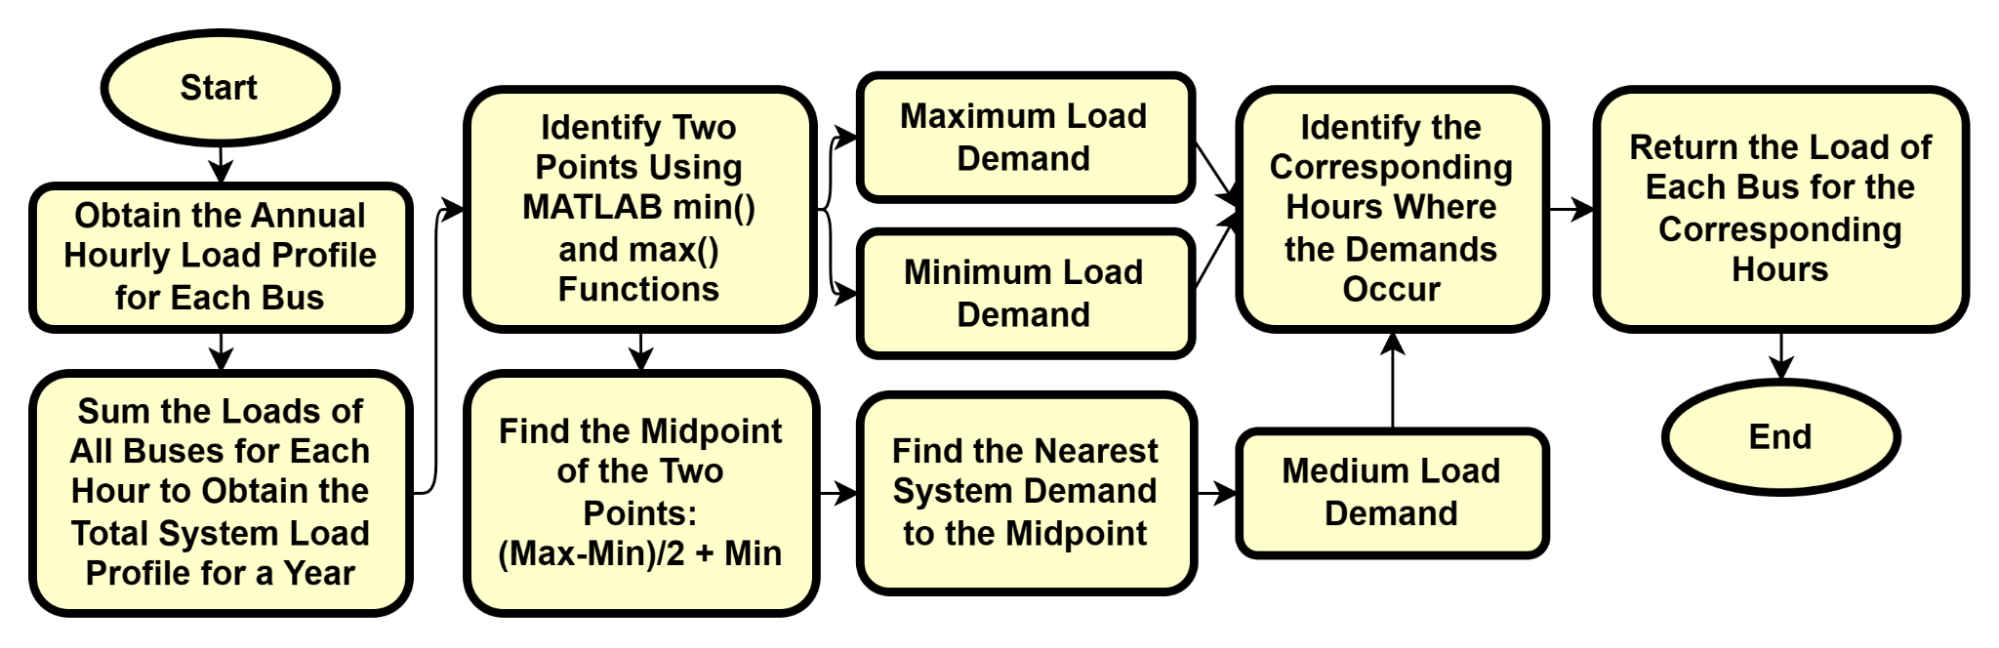
\includegraphics[width=0.9\textwidth]{multilevelflowchart.png}}
		\caption{3-Hour Load Profile Development Flowchart.}
		\label{fig:3hourchartdev}
	\end{figure}
	
	
	\begin{table}[htbp]
		\centering
		\caption{Load Demand of 33 Buses for 3 Hours}
		\vspace{10pt}
		\label{tab:3hoursloadprofile}
		\tiny % Reduce font size
		\setlength{\tabcolsep}{5pt}
		\resizebox{\textwidth}{!}{%
			\begin{tabular}{|c|ccc|ccc|}
				\hline
				\textbf{} & \multicolumn{3}{c|}{\textbf{P (kW)}}                                   & \multicolumn{3}{c|}{\textbf{Q (kVAr)}}                                  \\ \hline
				\textbf{Bus} &
				\multicolumn{1}{c|}{\textbf{Hour 1}} &
				\multicolumn{1}{c|}{\textbf{Hour 2}} &
				\textbf{Hour 3} &
				\multicolumn{1}{c|}{\textbf{Hour 1}} &
				\multicolumn{1}{c|}{\textbf{Hour 2}} &
				\textbf{Hour 3} \\ \hline
				1         & \multicolumn{1}{c|}{0}       & \multicolumn{1}{c|}{0}       & 0        & \multicolumn{1}{c|}{0}       & \multicolumn{1}{c|}{0}        & 0        \\ \hline
				2         & \multicolumn{1}{c|}{8.4858}  & \multicolumn{1}{c|}{64.4516} & 96.4926  & \multicolumn{1}{c|}{5.0915}  & \multicolumn{1}{c|}{38.6709}  & 57.8956  \\ \hline
				3         & \multicolumn{1}{c|}{8.935}   & \multicolumn{1}{c|}{48.282}  & 86.8396  & \multicolumn{1}{c|}{3.9711}  & \multicolumn{1}{c|}{21.4587}  & 38.5954  \\ \hline
				4         & \multicolumn{1}{c|}{7.8811}  & \multicolumn{1}{c|}{41.2028} & 128.6932 & \multicolumn{1}{c|}{5.2541}  & \multicolumn{1}{c|}{27.4685}  & 85.7955  \\ \hline
				5         & \multicolumn{1}{c|}{8.5614}  & \multicolumn{1}{c|}{57.998}  & 72.0976  & \multicolumn{1}{c|}{4.2807}  & \multicolumn{1}{c|}{28.999}   & 36.0488  \\ \hline
				6         & \multicolumn{1}{c|}{7.6754}  & \multicolumn{1}{c|}{57.9392} & 91.2525  & \multicolumn{1}{c|}{2.5585}  & \multicolumn{1}{c|}{19.3131}  & 30.4175  \\ \hline
				7         & \multicolumn{1}{c|}{8.7167}  & \multicolumn{1}{c|}{44.3225} & 90.7906  & \multicolumn{1}{c|}{4.3584}  & \multicolumn{1}{c|}{22.1613}  & 45.3953  \\ \hline
				8         & \multicolumn{1}{c|}{13.0079} & \multicolumn{1}{c|}{60.0554} & 82.3049  & \multicolumn{1}{c|}{6.5039}  & \multicolumn{1}{c|}{30.0277}  & 41.1524  \\ \hline
				9         & \multicolumn{1}{c|}{15.4558} & \multicolumn{1}{c|}{33.7835} & 34.2916  & \multicolumn{1}{c|}{5.1519}  & \multicolumn{1}{c|}{11.2612}  & 11.4305  \\ \hline
				10        & \multicolumn{1}{c|}{18.101}  & \multicolumn{1}{c|}{42.1559} & 76.0445  & \multicolumn{1}{c|}{6.0337}  & \multicolumn{1}{c|}{14.052}   & 25.3482  \\ \hline
				11        & \multicolumn{1}{c|}{9.1366}  & \multicolumn{1}{c|}{39.2378} & 87.0537  & \multicolumn{1}{c|}{6.0911}  & \multicolumn{1}{c|}{26.1585}  & 58.0358  \\ \hline
				12        & \multicolumn{1}{c|}{13.285}  & \multicolumn{1}{c|}{75.9815} & 80.9403  & \multicolumn{1}{c|}{7.7496}  & \multicolumn{1}{c|}{44.3225}  & 47.2151  \\ \hline
				13        & \multicolumn{1}{c|}{11.828}  & \multicolumn{1}{c|}{47.6354} & 131.4014 & \multicolumn{1}{c|}{6.8997}  & \multicolumn{1}{c|}{27.7873}  & 76.6508  \\ \hline
				14        & \multicolumn{1}{c|}{11.131}  & \multicolumn{1}{c|}{45.1665} & 73.3362  & \multicolumn{1}{c|}{7.4207}  & \multicolumn{1}{c|}{30.111}   & 48.8908  \\ \hline
				15        & \multicolumn{1}{c|}{10.1065} & \multicolumn{1}{c|}{35.5092} & 131.4854 & \multicolumn{1}{c|}{1.6844}  & \multicolumn{1}{c|}{5.9182}   & 21.9142  \\ \hline
				16        & \multicolumn{1}{c|}{12.0086} & \multicolumn{1}{c|}{88.876}  & 97.0594  & \multicolumn{1}{c|}{4.0029}  & \multicolumn{1}{c|}{29.6253}  & 32.3531  \\ \hline
				17        & \multicolumn{1}{c|}{10.8371} & \multicolumn{1}{c|}{39.1664} & 127.7695 & \multicolumn{1}{c|}{3.6124}  & \multicolumn{1}{c|}{13.0555}  & 42.5898  \\ \hline
				18        & \multicolumn{1}{c|}{16.9128} & \multicolumn{1}{c|}{62.0792} & 88.2     & \multicolumn{1}{c|}{7.5168}  & \multicolumn{1}{c|}{27.5908}  & 39.2     \\ \hline
				19        & \multicolumn{1}{c|}{10.4592} & \multicolumn{1}{c|}{51.851}  & 84.7486  & \multicolumn{1}{c|}{4.6485}  & \multicolumn{1}{c|}{23.0449}  & 37.666   \\ \hline
				20        & \multicolumn{1}{c|}{7.1757}  & \multicolumn{1}{c|}{49.4661} & 67.714   & \multicolumn{1}{c|}{3.1892}  & \multicolumn{1}{c|}{21.9849}  & 30.0951  \\ \hline
				21        & \multicolumn{1}{c|}{13.1003} & \multicolumn{1}{c|}{48.853}  & 60.2822  & \multicolumn{1}{c|}{5.8223}  & \multicolumn{1}{c|}{21.7125}  & 26.7921  \\ \hline
				22        & \multicolumn{1}{c|}{9.4095}  & \multicolumn{1}{c|}{62.243}  & 121.2403 & \multicolumn{1}{c|}{4.182}   & \multicolumn{1}{c|}{27.6636}  & 53.8846  \\ \hline
				23        & \multicolumn{1}{c|}{11.6601} & \multicolumn{1}{c|}{69.3096} & 77.556   & \multicolumn{1}{c|}{6.4778}  & \multicolumn{1}{c|}{38.5053}  & 43.0867  \\ \hline
				24        & \multicolumn{1}{c|}{14.0828} & \multicolumn{1}{c|}{44.9355} & 184.7052 & \multicolumn{1}{c|}{6.7061}  & \multicolumn{1}{c|}{21.3979}  & 87.9548  \\ \hline
				25        & \multicolumn{1}{c|}{9.3423}  & \multicolumn{1}{c|}{66.1521} & 82.6492  & \multicolumn{1}{c|}{4.4487}  & \multicolumn{1}{c|}{31.501}   & 39.3567  \\ \hline
				26        & \multicolumn{1}{c|}{7.2933}  & \multicolumn{1}{c|}{62.2094} & 75.2971  & \multicolumn{1}{c|}{3.0389}  & \multicolumn{1}{c|}{25.9206}  & 31.3738  \\ \hline
				27        & \multicolumn{1}{c|}{9.2206}  & \multicolumn{1}{c|}{49.0966} & 60.1898  & \multicolumn{1}{c|}{3.8419}  & \multicolumn{1}{c|}{20.4569}  & 25.0791  \\ \hline
				28        & \multicolumn{1}{c|}{10.1653} & \multicolumn{1}{c|}{42.1266} & 94.2966  & \multicolumn{1}{c|}{3.3884}  & \multicolumn{1}{c|}{14.0422}  & 31.4322  \\ \hline
				29        & \multicolumn{1}{c|}{11.8322} & \multicolumn{1}{c|}{39.6073} & 93.4653  & \multicolumn{1}{c|}{6.9021}  & \multicolumn{1}{c|}{23.1042}  & 54.5214  \\ \hline
				30        & \multicolumn{1}{c|}{17.341}  & \multicolumn{1}{c|}{55.6383} & 155.4479 & \multicolumn{1}{c|}{52.0231} & \multicolumn{1}{c|}{166.9149} & 466.3438 \\ \hline
				31        & \multicolumn{1}{c|}{7.9777}  & \multicolumn{1}{c|}{32.4651} & 110.6761 & \multicolumn{1}{c|}{3.7229}  & \multicolumn{1}{c|}{15.1504}  & 51.6489  \\ \hline
				32        & \multicolumn{1}{c|}{8.2338}  & \multicolumn{1}{c|}{67.3487} & 77.2579  & \multicolumn{1}{c|}{3.9209}  & \multicolumn{1}{c|}{32.0708}  & 36.7895  \\ \hline
				33        & \multicolumn{1}{c|}{12.2563} & \multicolumn{1}{c|}{50.8349} & 78.421   & \multicolumn{1}{c|}{8.1709}  & \multicolumn{1}{c|}{33.8899}  & 52.2806  \\ \hline
			\end{tabular}%
		}
	\end{table}
	
	\subsubsection{Daily Load Demand (24 Hours)}
	The daily load profile consists of 24 hours of load data for the system. To determine this load profile, we first assumed that demand on weekdays and weekends did not differ significantly. Figure~\ref{fig:24hourchartdev} illustrates the process of extracting a representative daily load profile. The detailed load of each bus for 24 hours could be accessed through the supplementary materials titled \href{https://docs.google.com/spreadsheets/d/1aUaok1M9MFdV-2YwGXDtjuIwCXB-yF1H/edit?usp=sharing&ouid=104271507204643812053&rtpof=true&sd=true}{Appendix\_Daily\_Load\_P\_Data.xlsx} and \href{https://docs.google.com/spreadsheets/d/1owMe5SsF_vXdNSdqBIJJ5x3NKYC_CiQ1/edit?usp=sharing&ouid=104271507204643812053&rtpof=true&sd=true}{Appendix\_Daily\_Load\_Q\_Data.xlsx}.
	
	
	\begin{figure}[htbp]
		\centerline{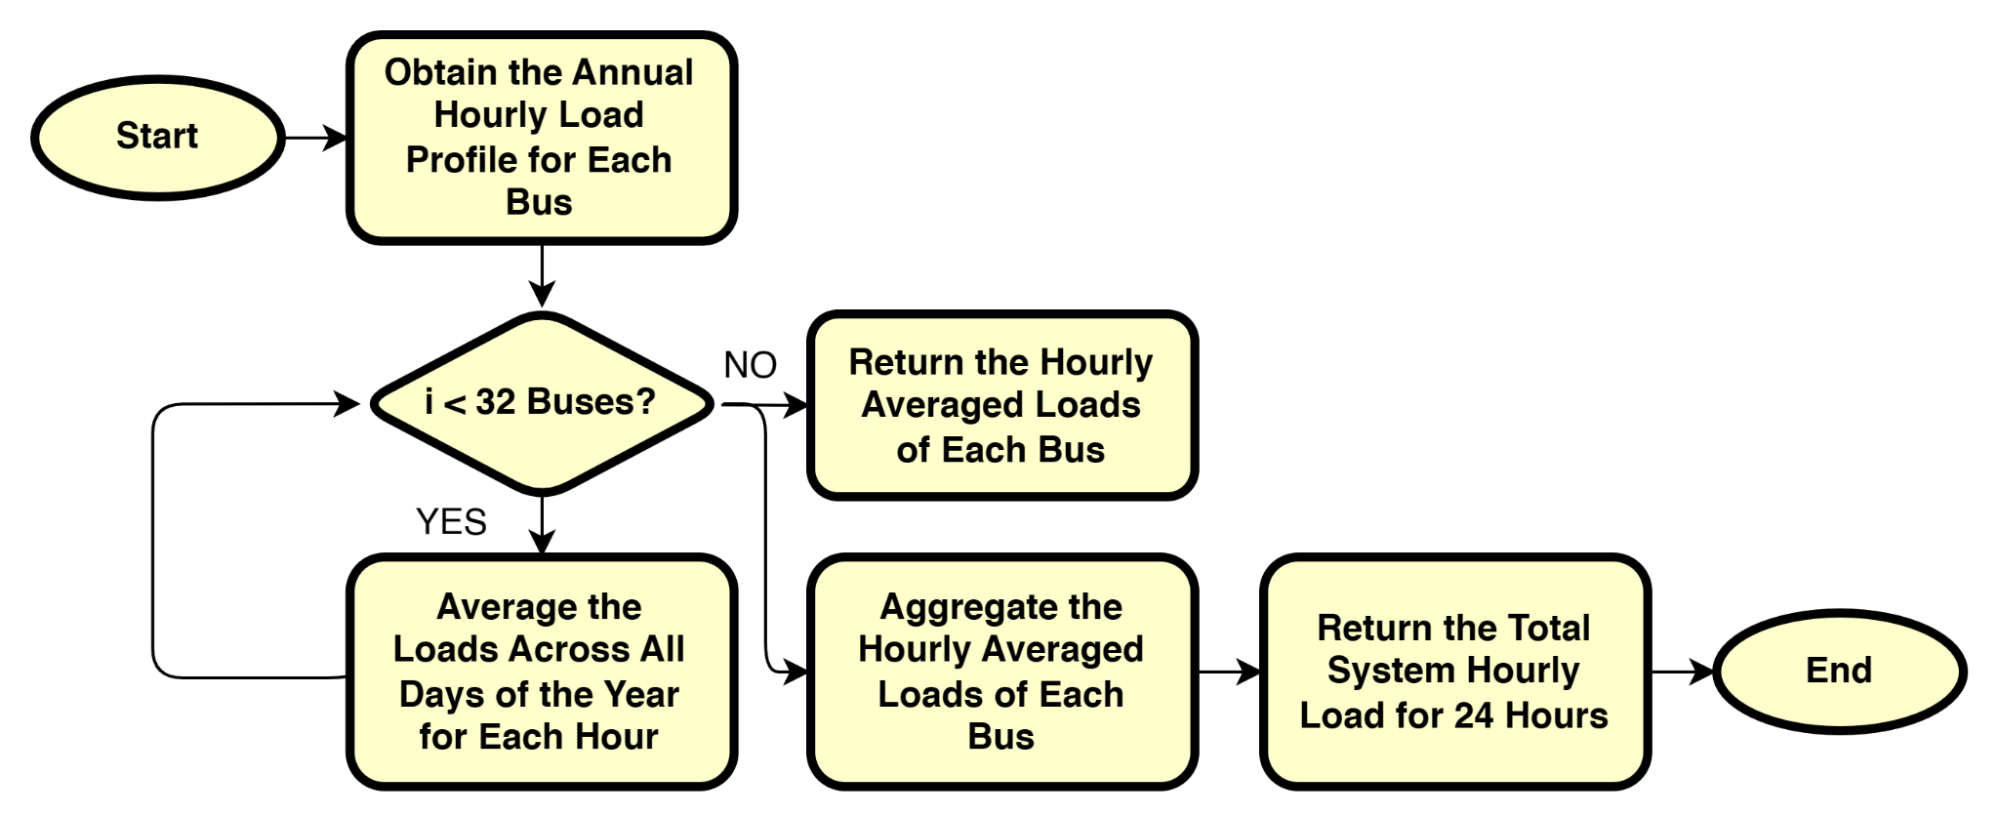
\includegraphics[width=0.9\textwidth]{dailychart.png}}
		\caption{24-Hour Load Profile Development Flowchart.}
		\label{fig:24hourchartdev}
	\end{figure}
	
	
	\subsubsection{Seasonal Load Demand (96 Hours)}
	We condensed four seasons into a 96-hour load profile, where each season is represented in a 24-hour period. Figure \ref{fig:96hourchartdev} provides an illustration of how the seasonal load profiles are developed. The detailed load of each bus for 96 hours could be accessed through the supplementary materials titled \href{https://docs.google.com/spreadsheets/d/1aUaok1M9MFdV-2YwGXDtjuIwCXB-yF1H/edit?usp=sharing&ouid=104271507204643812053&rtpof=true&sd=true}{Appendix\_Seasonal\_Load\_P\_Data.xlsx} and \href{https://docs.google.com/spreadsheets/d/12WRgx53A4gAkal306UHPLYaDwVpHLaF3/edit?usp=sharing&ouid=104271507204643812053&rtpof=true&sd=true}{Appendix\_Seasonal\_Load\_Q\_Data.xlsx}.
	
	\begin{figure}[htbp]
		\centerline{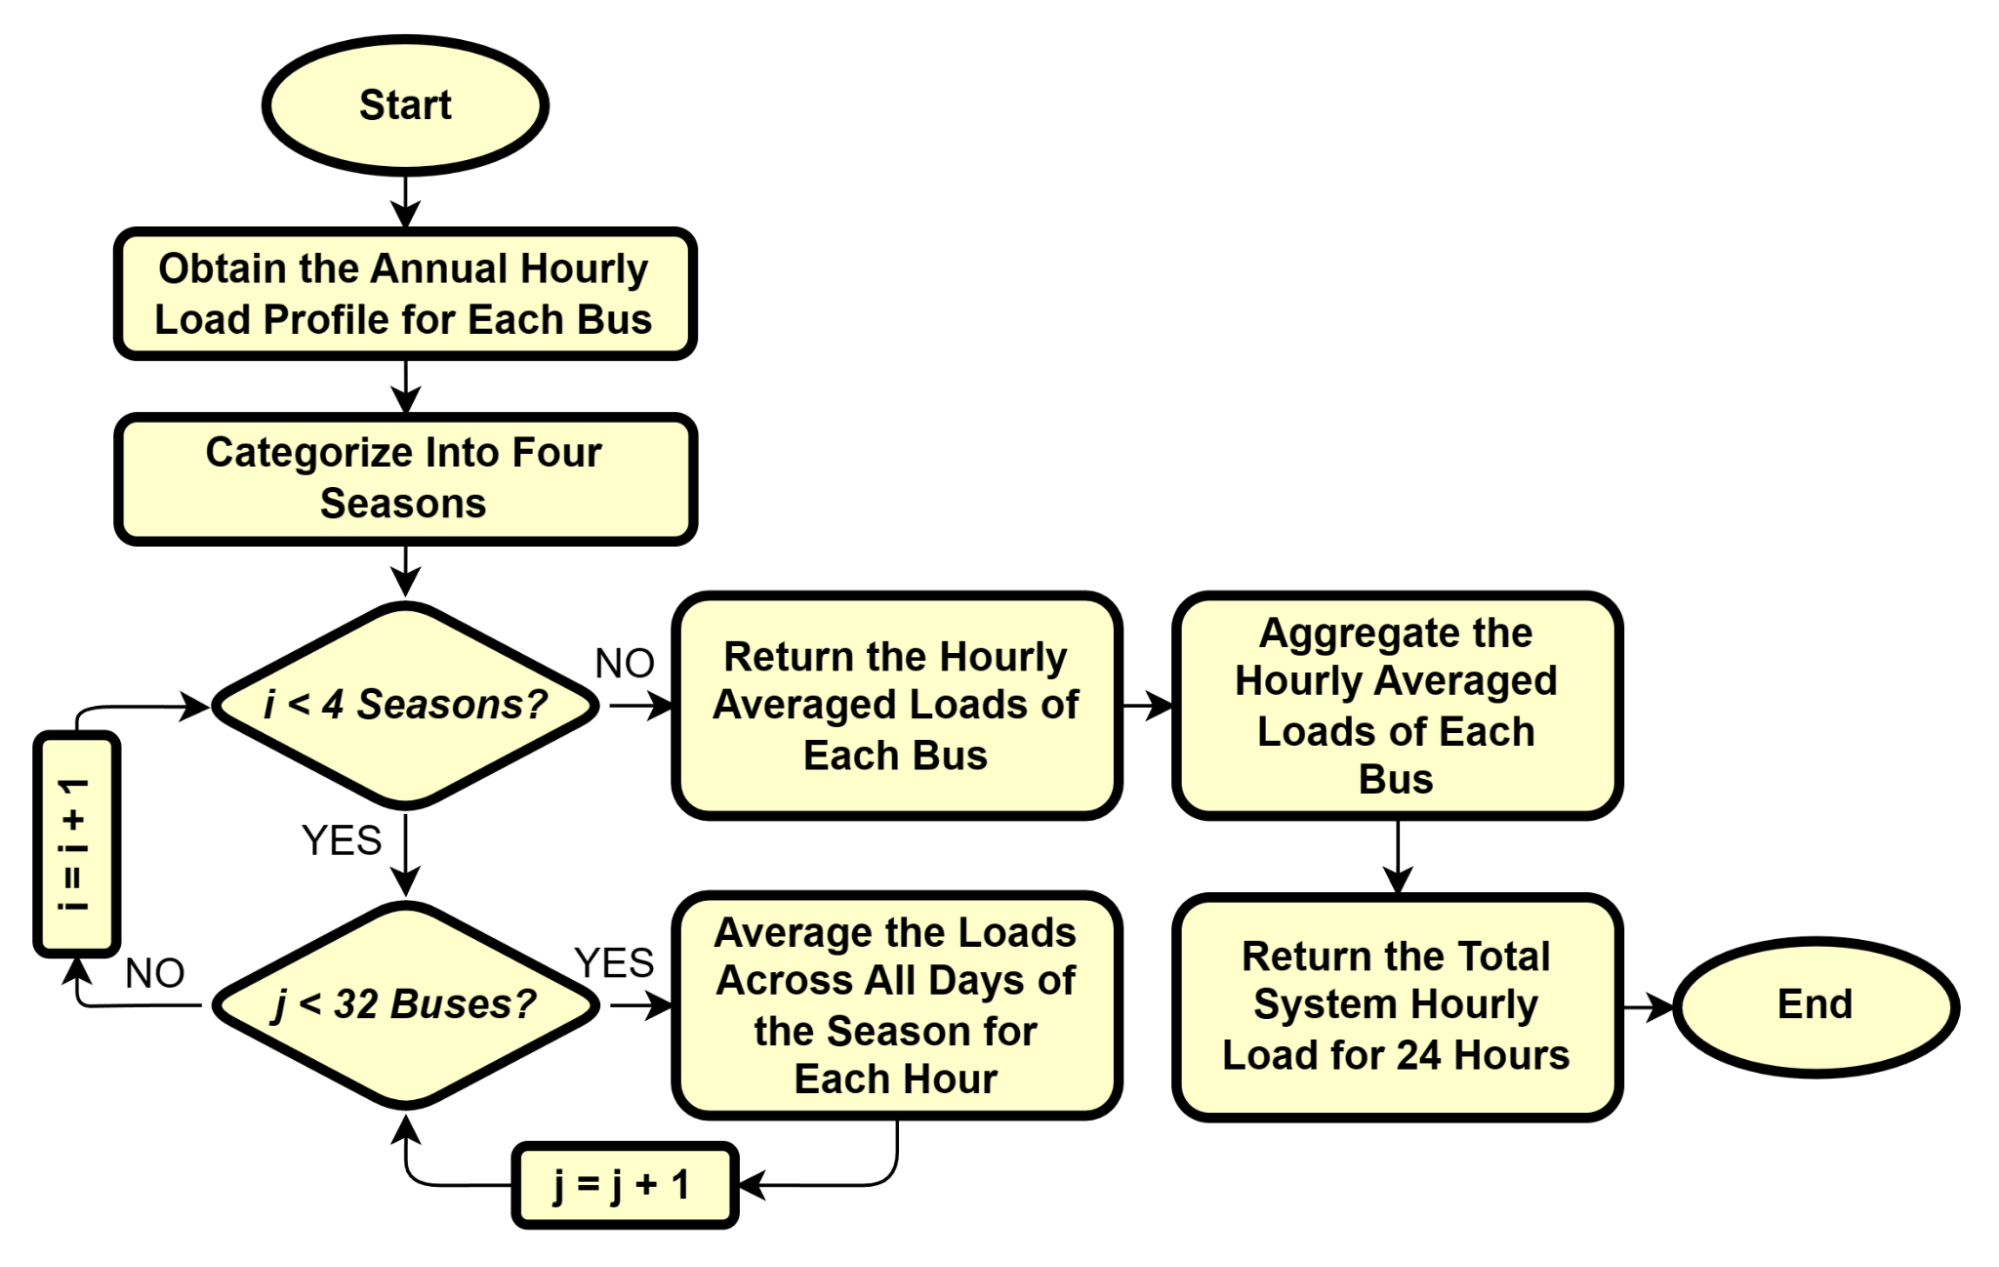
\includegraphics[width=0.9\textwidth]{96hourchart.png}}
		\caption{96-Hour Load Profile Development Flowchart.}
		\label{fig:96hourchartdev}
	\end{figure}
	
	\section{Results Data}
	This section details the bus and line data used in the study.
	
	\subsection{Comparison of Published Results For Single DG Integration}
	
	Table~\ref{tab:singleDGcomparison} presents the optimal allocation of a DG with the corresponding power losses from studies conducted until 2016. Results indicate that both WOA and E-WOA are effective optimizers for this problem.
	
	\begin{table}[htbp]
		\caption{Optimization Results for Single DG in IEEE 33-Bus System at Unity Power Factor}
		%	\vspace{-20pt}
		\begin{center}
			\resizebox{\columnwidth}{!}{%
				\begin{tabular}{ccccc}
					\hline
					\textbf{Year} &
					\textbf{Algorithm} &
					\textbf{\begin{tabular}[c]{@{}c@{}}DG \\ Location\end{tabular}} &
					\textbf{\begin{tabular}[c]{@{}c@{}}DG Size\\  (kW)\end{tabular}} &
					\textbf{Power Loss (kW)} \\ \hline
					\multicolumn{2}{c}{Base}             & -          & -                 & 210.988          \\
					2016$^{\mathrm{a}}$             & BFOA           & 6          & 2200.000          & 113.140          \\
					2016$^{\mathrm{b}}$            & HSA-PABC       & 6          & 2598.000          & 111.030          \\
					2017$^{\mathrm{c}}$            & GWO            & 6          & 2761.820          & 111.420          \\
					2018$^{\mathrm{d}}$             & GA             & 6          & 2600.000          & 111.030          \\
					2018$^{\mathrm{e}}$             & DA             & 6          & 2590.200          & 111.034          \\
					2021$^{\mathrm{f}}$            & MRFO           & 6          & 2590.217          & 111.027          \\
					2021$^{\mathrm{g}}$            & PFA            & 6          & 2590.264          & 111.030          \\
					2022$^{\mathrm{h}}$             & HBA            & 30         & 1542.000          & 125.000          \\
					\textbf{Present} & \textbf{WOA}   & \textbf{6} & \textbf{2590.217} & \textbf{111.019} \\
					\textbf{Present} & \textbf{E-WOA} & \textbf{6} & \textbf{2590.217} & \textbf{111.019} \\ \hline
					\multicolumn{5}{l}{$^{\mathrm{a}}${\scriptsize Devabalaji et al., 2016.}} \\
					\multicolumn{5}{l}{$^{\mathrm{b}}${\scriptsize Muthukumar et al., 2016.}} \\
					\multicolumn{5}{l}{$^{\mathrm{c}}${\scriptsize El-Sayed et al., 2017.}} \\
					\multicolumn{5}{l}{$^{\mathrm{d}}${\scriptsize Kashyap et al., 2018.}} \\
					\multicolumn{5}{l}{$^{\mathrm{e}}${\scriptsize Suresh et al., 2018.}} \\
					\multicolumn{5}{l}{$^{\mathrm{f}}${\scriptsize Hemeida et al., 2021.}} \\
					\multicolumn{5}{l}{$^{\mathrm{g}}${\scriptsize Janamala, 2021.}} \\
					\multicolumn{5}{l}{$^{\mathrm{h}}${\scriptsize Khan, 2022.}} \\
				\end{tabular}%
			}
			\label{tab:singleDGcomparison}
		\end{center}
	\end{table}
	
	\subsection{Optimization Algorithm}
	\subsubsection{Whale Optimization Algorithm (WOA)}
	
	Fig. \ref{fig:WOAflowchart} presents the optimal flowchart of WOA including the modifications implemented for solving the mixed-integer ODGA problem.
	
	\begin{figure}[htbp]
		\centerline{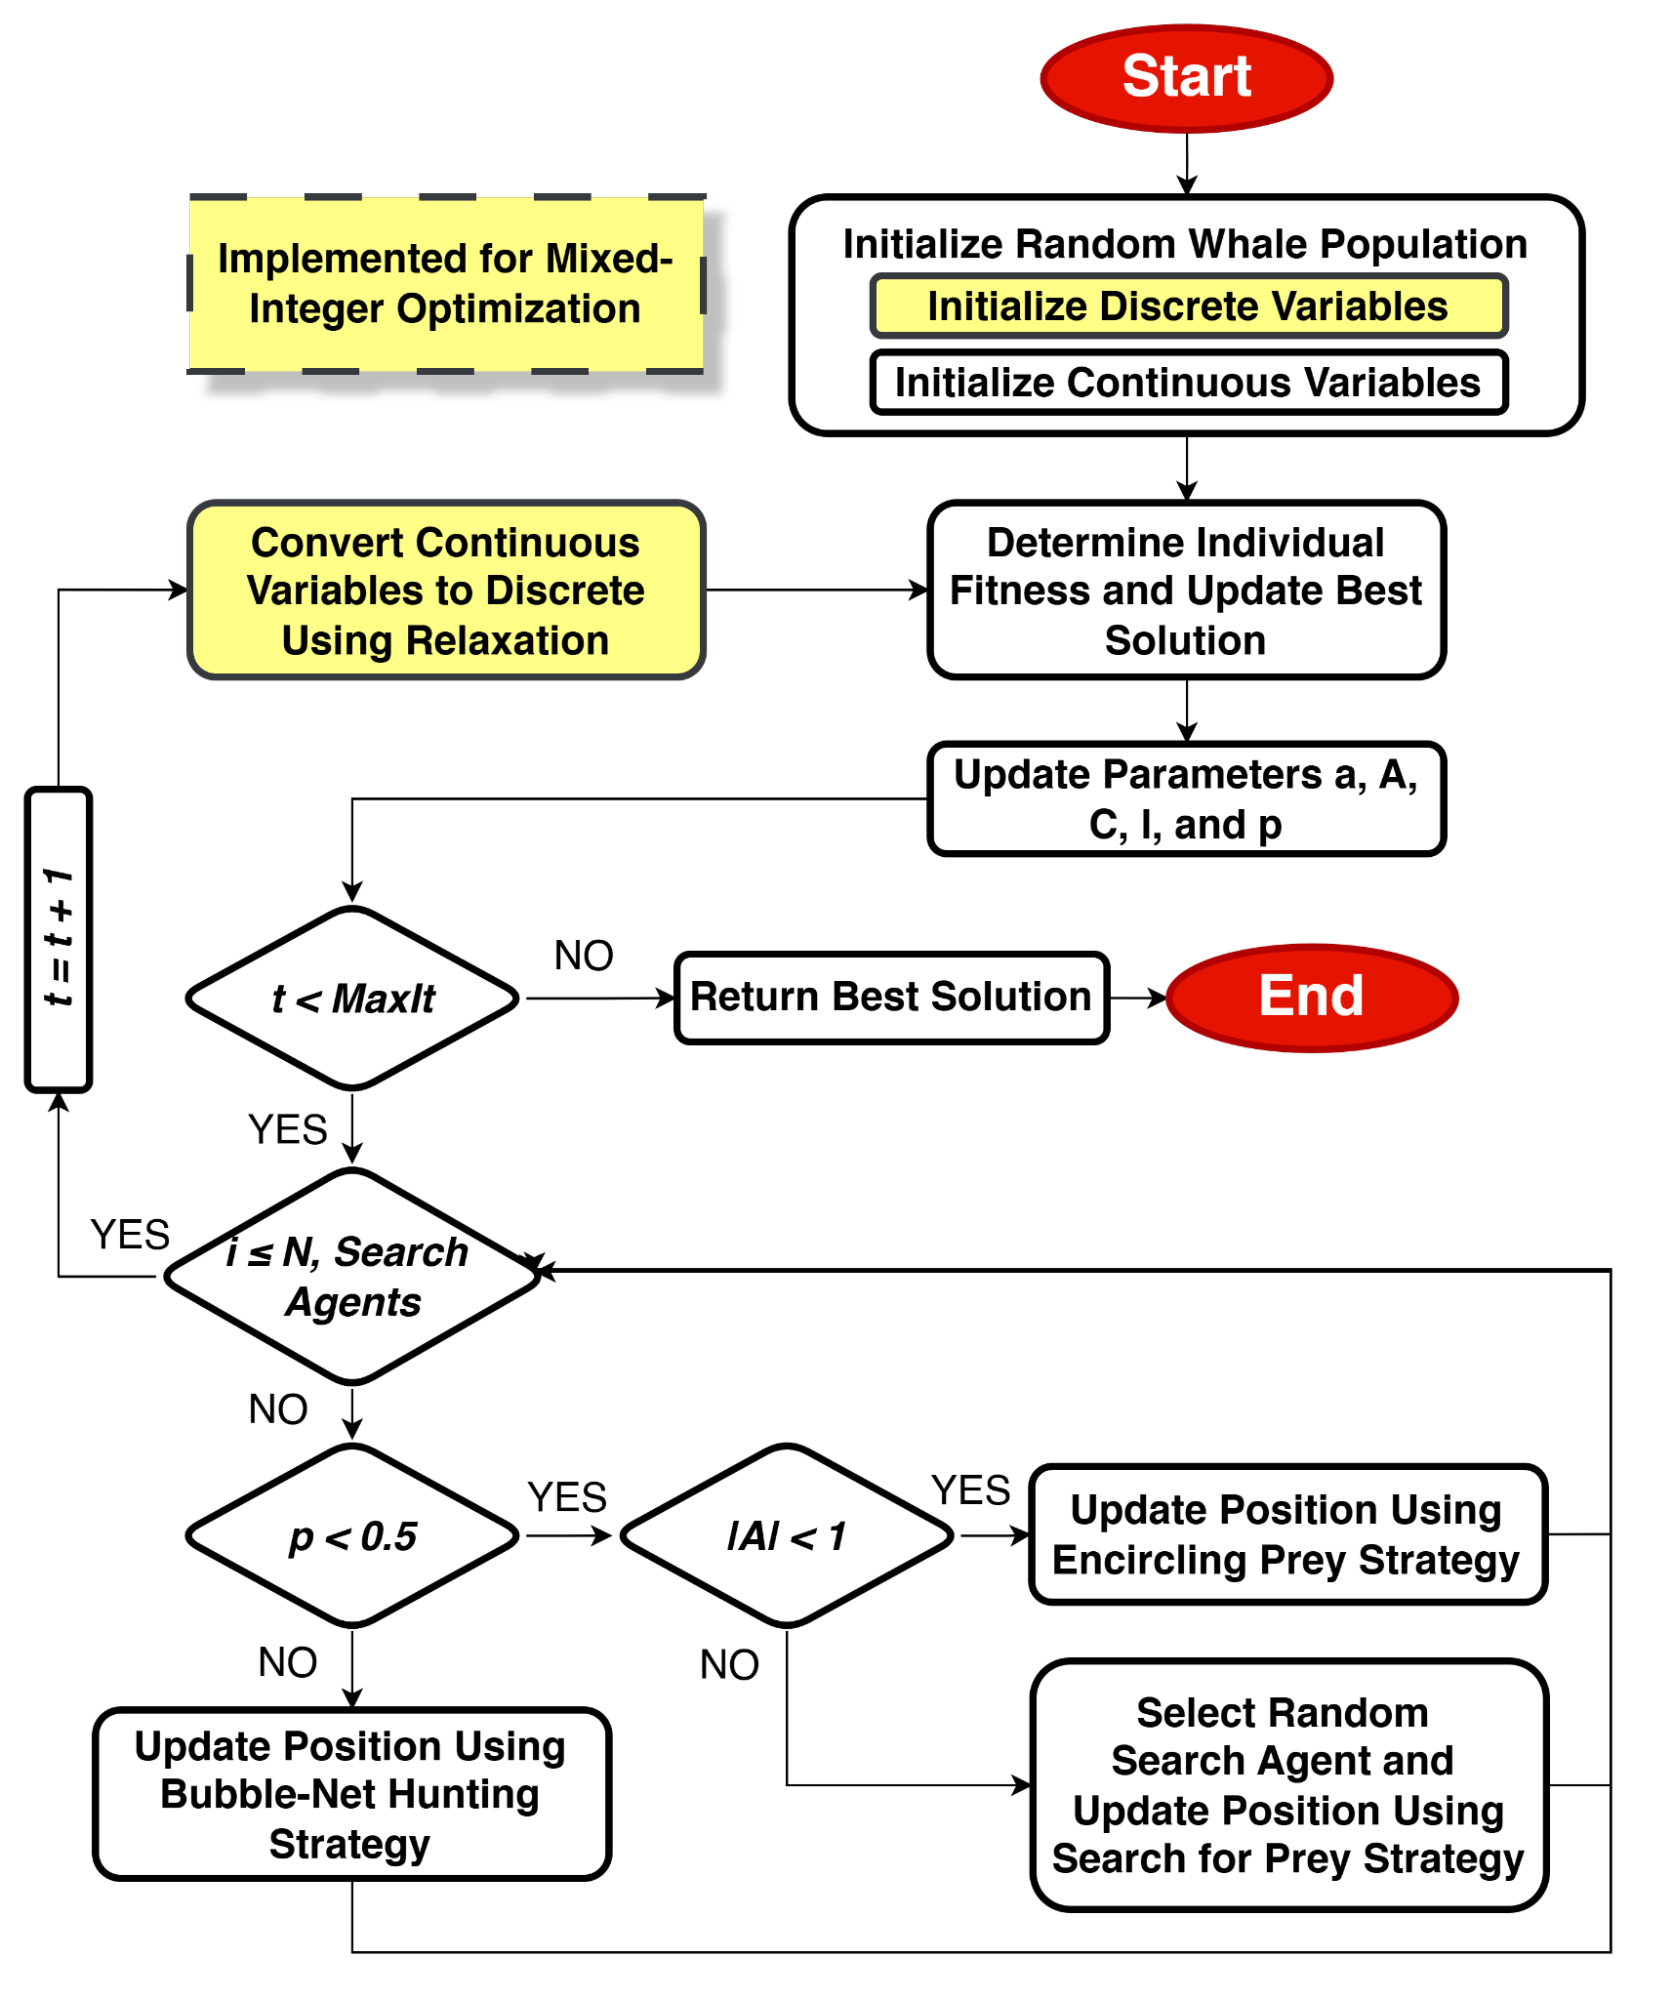
\includegraphics[width=0.9\textwidth]{WOAflowchart.png}}
		\caption{Whale Optimization Algorithm Flowchart.}
		\label{fig:WOAflowchart}
	\end{figure}
	
	\subsection{Convergence Curves}
	The following figures illustrate the convergence curves of WOA and E-WOA for 100 runs as well as the comparison of their best convergence curves.
	
	
	\subsubsection{Case 1 Comparison}
	
	Fig. \ref{fig:case1convcomp} presents the comparison of the best convergence curve of each algorithm for Case 1.
	
	\begin{figure}[htbp]
		\centerline{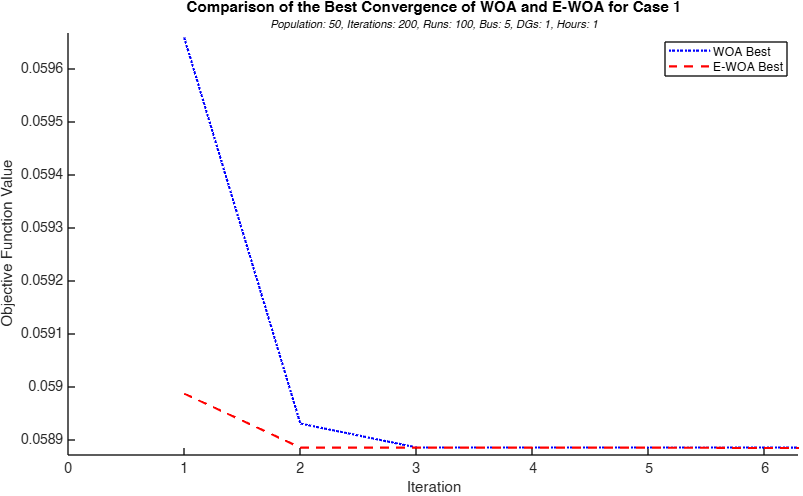
\includegraphics[width=0.7\textwidth]{case1comp.png}}
		\caption{Comparison of Best Convergence Curves for Case 1.}
		\label{fig:case1convcomp}
	\end{figure}
	
	\subsubsection{Case 2 Comparison}
	
	Fig. \ref{fig:case2convcomp} presents the comparison of the best convergence curve of each algorithm for Case 2.
	
	\begin{figure}[htbp]
		\centerline{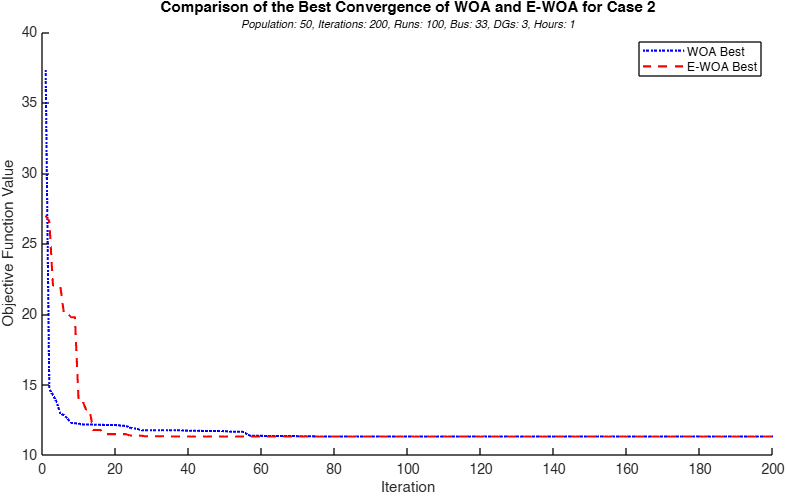
\includegraphics[width=0.7\textwidth]{case2comp.png}}
		\caption{Comparison of Best Convergence Curves for Case 2.}
		\label{fig:case2convcomp}
	\end{figure}
	
	\subsubsection{Case 3 Comparison}
	
	Fig. \ref{fig:case3convcomp} presents the comparison of the best convergence curve of each algorithm for Case 3.
	
	\begin{figure}[htbp]
		\centerline{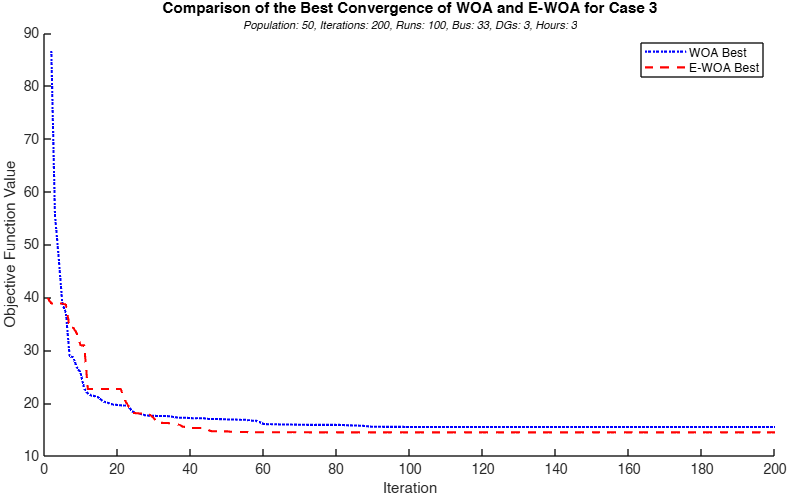
\includegraphics[width=0.7\textwidth]{case3comp.png}}
		\caption{Comparison of Best Convergence Curves for Case 3.}
		\label{fig:case3convcomp}
	\end{figure}
	
	\subsubsection{Case 5 Comparison}
	
	Fig. \ref{fig:case5convcomp} presents the comparison of the best convergence curve of each algorithm for Case 5. Since E-WOA failed to find any feasible solutions in 100 runs, only WOA's convergence curve is shown.
	
	\begin{figure}[htbp]
		\centerline{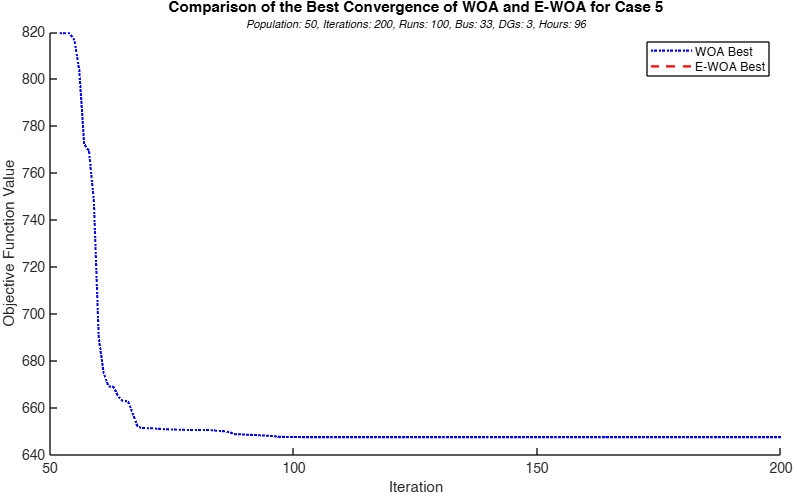
\includegraphics[width=0.7\textwidth]{case5comp.png}}
		\caption{Comparison of Best Convergence Curves for Case 5.}
		\label{fig:case5convcomp}
	\end{figure}

	
\end{document}



